% =============================================================================
\section{Cuando algo no jala}
% =============================================================================

\begin{frame}{Revisa en este orden}
  \centering
  \begin{tikzpicture}[every node/.style={font=\scriptsize,align=center},
      q/.style={draw=azul,fill=azulclaro,rounded corners,text width=2.35cm,minimum height=1.25cm},
      f/.style={draw=rojo,fill=red!5,rounded corners,text width=2.35cm,minimum height=0.9cm,font=\tiny}]
    \node[q] (a) at (0,0) {\textbf{1} ¿\cmd{vespo doctor} sale todo en verde?};
    \node[q] (b) at (2.75,0) {\textbf{2} ¿Aparecen los topics \cmd{/fmu}?};
    \node[q] (c) at (5.5,0) {\textbf{3} ¿\cmd{telemetry\_listener} recibe datos?};
    \node[q] (d) at (8.25,0) {\textbf{4} ¿QGC dice \textbf{Ready To Fly}?};
    \node[q] (e) at (11,0) {\textbf{5} ¿En qué \textbf{modo} está? ¿Qué dice el monitor?};
    \foreach \x/\y in {a/b,b/c,c/d,d/e} \draw[-{Stealth},thick,verde] (\x) -- node[above,font=\tiny]{sí} (\y);
    \node[f] (fa) at (0,-1.9) {corre el \cmd{fix} que te dice};
    \node[f] (fb) at (2.75,-1.9) {¿corre el agente? \cmd{vespo down} y \cmd{vespo up -{}-sim}};
    \node[f] (fc) at (5.5,-1.9) {¿mismo \cmd{ROS\_DOMAIN\_ID}? ¿PX4 arrancó?};
    \node[f] (fd) at (8.25,-1.9) {lee el mensaje rojo de QGC; espera al GPS};
    \node[f] (fe) at (11,-1.9) {\cmd{flight\_mode\_monitor} dice qué hizo PX4};
    \foreach \x in {a,b,c,d,e} \draw[-{Stealth},thick,rojo] (\x) -- node[right,font=\tiny]{no} (f\x);
  \end{tikzpicture}
  \vspace{0.5em}

  \raggedright\small Casi siempre el problema está en el \textbf{primer} paso que falla. No te saltes pasos:
  revisar tu código cuando el agente ni siquiera corre es tiempo perdido.
\end{frame}

\begin{frame}{Síntoma, causa, arreglo (1/2)}
  \centering\scriptsize
  \begin{tabular}{p{4.1cm}p{4.3cm}p{4.6cm}}
    \toprule
    Ves & Casi siempre es & Haz \\
    \midrule
    \cmd{ros2 topic list} no tiene \cmd{/fmu} & el agente no corre & \cmd{vespo up -{}-sim} (o \cmd{vespo agent}) \\
    Tu nodo no recibe nada, sin error & nombre sin \cmd{\_v1}, o QoS \cmd{reliable} & copia nombre y QoS de un ejemplo \\
    \cmd{No executable found} & no compilaste, o paquete nuevo & \cmd{vespo build} y terminal nueva \\
    Cambiaste el código y hace lo mismo & no compilaste (o falló el build) & \cmd{vespo build}, lee los errores \\
    \cmd{UDP port 8888 busy} & quedó algo de antes & \cmd{vespo down} \\
    Gazebo lentísimo o la laptop se apaga & batería, o un proceso zombi & cargador; \cmd{vespo down} \\
    \bottomrule
  \end{tabular}
\end{frame}

\begin{frame}{Síntoma, causa, arreglo (2/2): el dron}
  \centering\scriptsize
  \begin{tabular}{p{4.1cm}p{4.3cm}p{4.6cm}}
    \toprule
    Ves & Casi siempre es & Haz \\
    \midrule
    No arma: ``No connection to the GCS'' & QGroundControl cerrado & ábrelo (\cmd{vespo qgc}); \cmd{vespo up} ya lo abre \\
    No arma recién arrancado & el GPS o el estimador aún no están listos & espera a \textbf{Ready To Fly} \\
    No entra a Offboard & no hubo setpoints antes & calienta 1 s antes de pedir el modo \\
    Sube y luego pasa a \textbf{Hold} & tu nodo dejó de publicar (Ctrl+C, crash, un \cmd{sleep}) & \cmd{flight\_mode\_monitor} lo confirma \\
    Se va a otro lado & confundiste NED: \cmd{z} positivo es \textbf{abajo}; x es norte & revisa signos y orden \\
    Llega y nunca pasa al siguiente WP & tolerancia muy chica o WP inalcanzable & imprime la distancia al WP \\
    Se desarma solo en tierra & armó y nadie le pidió despegar & normal: es seguridad de PX4 \\
    \bottomrule
  \end{tabular}
\end{frame}

\begin{frame}[fragile]{La hoja para tener a la mano}
  \begin{columns}[t]
    \column{0.5\textwidth}
    \begin{lstlisting}[style=bash,caption={vespo}]
vespo doctor          # todo bien?
vespo update          # lo nuevo del equipo
vespo build [PKG]     # compilar
vespo up --sim        # simulacion completa
vespo up --sim --world plaza_show
vespo down            # apagar todo
vespo simulate --show # modelos y mundos
vespo config          # mi configuracion
    \end{lstlisting}
    \column{0.47\textwidth}
    \begin{lstlisting}[style=bash,caption={ROS 2}]
ros2 run px4_examples telemetry_listener
ros2 run px4_examples flight_mode_monitor
ros2 topic list | grep fmu
ros2 topic echo /fmu/out/vehicle_status_v1 \
  --field nav_state
ros2 interface show px4_msgs/msg/<Tipo>
    \end{lstlisting}
    \scriptsize\textbf{nav\_state}: 4 Hold · 14 Offboard · 17 Takeoff · 18 Land · 5 Return
  \end{columns}
\end{frame}

\begin{frame}{Y después}
  \begin{columns}[c]
    \column{0.52\textwidth}\small
    \begin{enumerate}
      \item Corre los 18 ejemplos, con \cmd{flight\_mode\_monitor} al lado.
      \item Haz los ejercicios de \cmd{square\_mission}.
      \item Resuelve la \textbf{estrella}.
      \item Sigue con los retos de \cmd{x500\_retos}: el pilar, la entrega, la geocerca, la cueva\ldots
    \end{enumerate}
    \vspace{0.3em}
    \begin{idea}
      \small ¿Dudas de un mensaje o de un ejemplo línea por línea? Está todo en la \textbf{referencia técnica}
      (\cmd{referencia.pdf}).
    \end{idea}
    \column{0.45\textwidth}\centering
    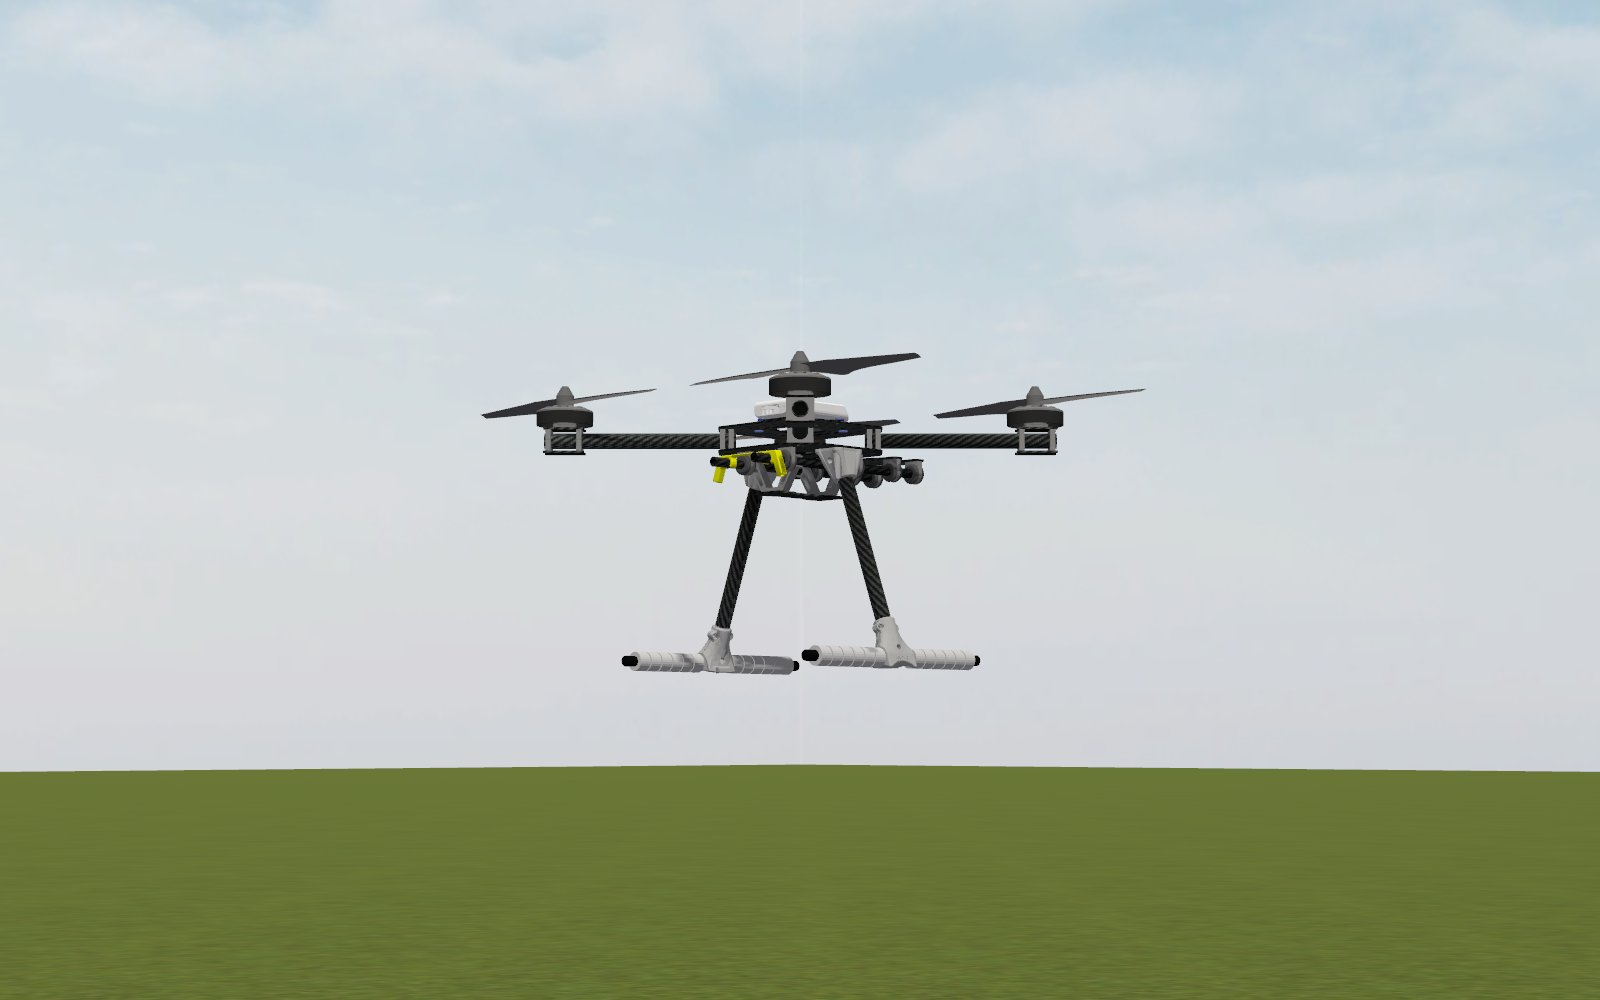
\includegraphics[width=\linewidth]{x500_volando}
  \end{columns}
\end{frame}
